\documentclass[11pt]{article}
\usepackage[margin=1in]{geometry}
\usepackage{amsmath,amssymb,amsthm}
\usepackage{graphicx}
\usepackage[colorlinks=true,linkcolor=blue,citecolor=blue,urlcolor=blue]{hyperref}

\newtheorem{theorem}{Theorem}
\newtheorem{lemma}{Lemma}

\newcommand{\R}{\mathbb{R}}
\newcommand{\PiRel}{\Pi}

\title{A Concrete Relative Projection Constant Equal to \texorpdfstring{\(7/3\)}{7/3}}
\author{Run \texttt{fa\_banach\_001}, lane \texttt{agent\_lane\_01}}
\date{2026-06-14}

\begin{document}
\maketitle

\section*{Source Problem}

This packet addresses the final question in Giuliano Basso's
\emph{Computation of maximal projection constants}, arXiv:1901.07866
\cite{Basso2019}.  In Remark 4.6, after listing
\[
  \PiRel(1,1)=1,\qquad
  \PiRel(2,3)=\frac43,\qquad
  \PiRel(4,6)=\frac53,\qquad
  \PiRel(5,10)=2,
\]
the source asks:
\[
  \text{Are there integers } n\le d \text{ such that }
  \PiRel(n,d)=\frac73?
\]
Here
\[
  \PiRel(n,d)=
  \sup\{\PiRel(E): E\subset \ell_\infty^d
  \text{ is an }n\text{-dimensional Banach space}\}.
\]

\begin{figure}[h]
\centering
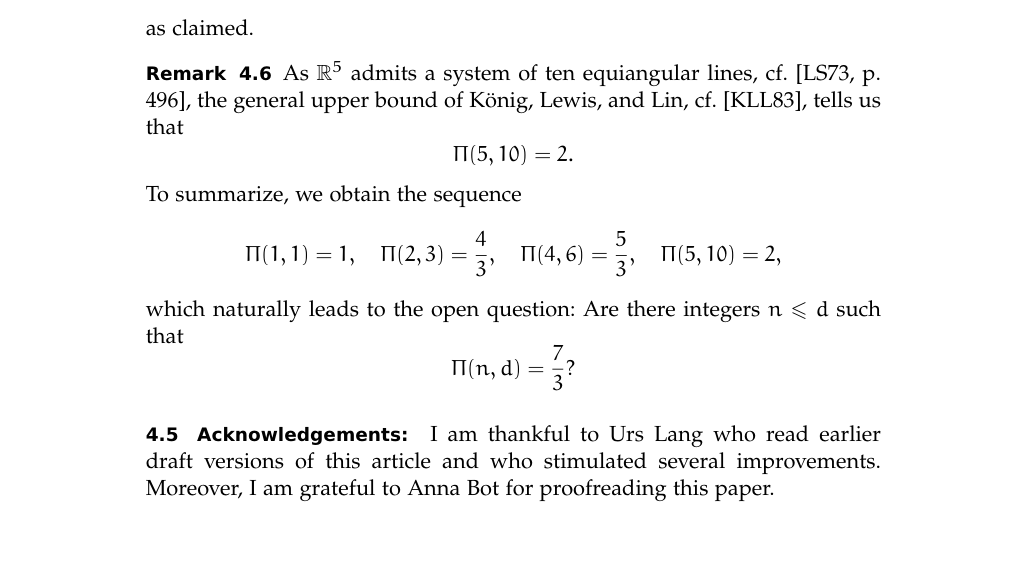
\includegraphics[width=0.92\textwidth]{figures/source_open_question_page24.png}
\caption{Basso, Remark 4.6, where the \(7/3\) question is posed.}
\end{figure}

\section*{Background Used}

The same source recalls the theorem of Koenig--Lewis--Lin \cite{KLL1983}:
\[
  \PiRel(n,d)\le
  \frac nd+\sqrt{(d-1)\frac nd\left(1-\frac nd\right)},
\]
with equality if and only if \(\R^n\) admits a system of \(d\) distinct
equiangular lines.

\begin{figure}[h]
\centering
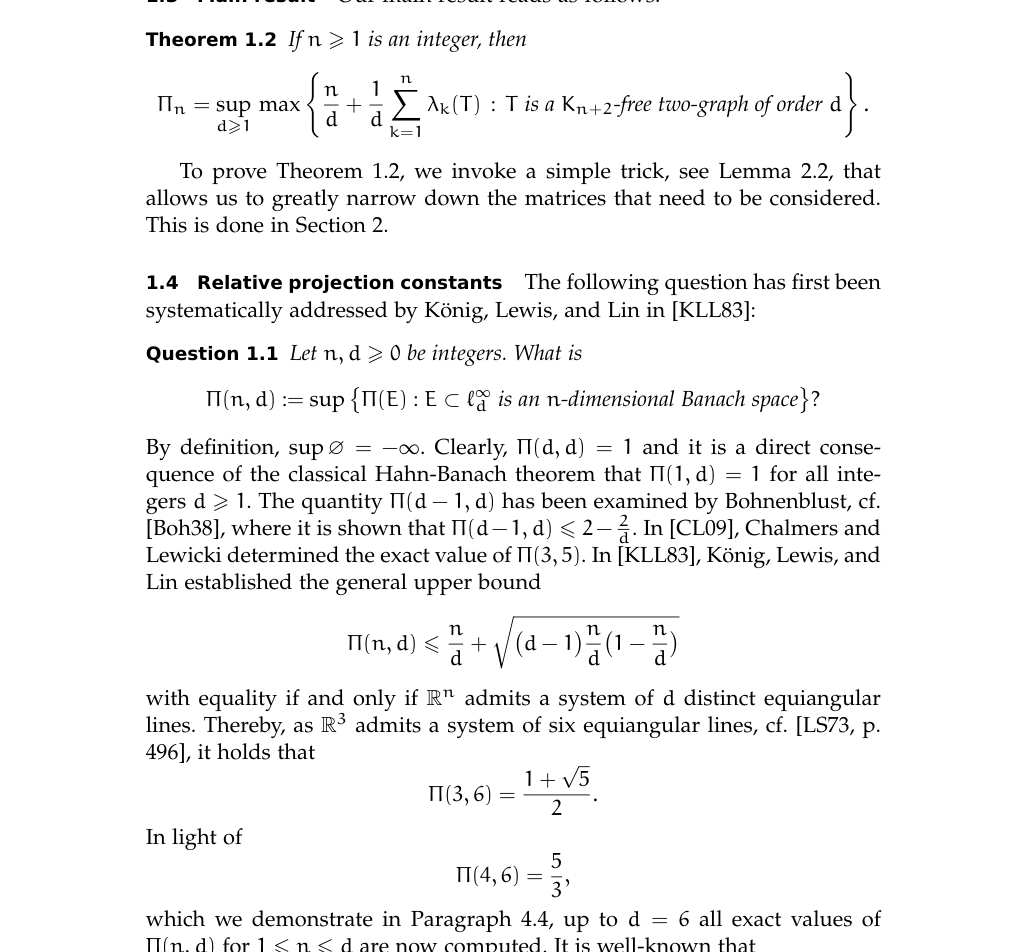
\includegraphics[width=0.92\textwidth]{figures/source_definition_kll_page4.png}
\caption{Basso's definition of \(\Pi(n,d)\) and the quoted
Koenig--Lewis--Lin equality criterion.}
\end{figure}

\section*{Proof Intuition}

The value \(7/3\) is forced by the Koenig--Lewis--Lin bound when
\((n,d)=(7,15)\):
\[
  \frac7{15}+
  \sqrt{14\cdot \frac7{15}\cdot \frac8{15}}
  =
  \frac7{15}+\frac{28}{15}
  =
  \frac73.
\]
So the problem reduces to a finite-dimensional geometric certificate:
produce 15 equiangular lines in a 7-dimensional real space.  The standard
28-line configuration in \(\R^7\) gives this immediately, and the explicit
model below keeps the reduction checkable.

\section*{The Answer}

\begin{theorem}
\[
  \PiRel(7,15)=\frac73.
\]
\end{theorem}

\begin{proof}
Let \(H=\{x\in \R^8:\sum_{k=1}^8 x_k=0\}\).  Then \(H\) is a
7-dimensional real Hilbert space.  For each two-element set
\(A=\{i,j\}\subset\{1,\ldots,8\}\), define
\[
  v_A=e_i+e_j-\frac14(1,1,1,1,1,1,1,1)\in H.
\]
For two such sets \(A\) and \(B\),
\[
  \langle v_A,v_B\rangle = |A\cap B|-\frac12.
\]
In particular, \(\|v_A\|^2=3/2\), and for \(A\ne B\) the absolute value of
\(\langle v_A,v_B\rangle\) is \(1/2\).  Thus the lines spanned by the
nonzero vectors \(v_A\) are equiangular, with common normalized absolute
inner product \((1/2)/(3/2)=1/3\).

Select the following 15 two-element sets:
\[
  \{1,j\}\ (2\le j\le 8),\qquad
  \{2,j\}\ (3\le j\le 8),\qquad
  \{3,4\},\{3,5\}.
\]
The first seven selected vectors \(v_{\{1,j\}}\), \(2\le j\le 8\), already
span \(H\).  Indeed, if
\[
  \sum_{j=2}^8 a_j v_{\{1,j\}}=0
\]
and \(A=\sum_{j=2}^8 a_j\), then the \(k\)-th coordinate for \(2\le k\le 8\)
gives \(a_k-A/4=0\).  Hence all \(a_k=A/4\), so
\[
  A=7A/4,
\]
which forces \(A=0\) and therefore \(a_k=0\) for all \(k\).  Since \(H\) has
dimension 7, these seven vectors are a basis of \(H\).

Consequently \(H\cong\R^7\) admits 15 distinct equiangular lines.  Applying
the Koenig--Lewis--Lin equality criterion quoted above,
\[
  \PiRel(7,15)
  =
  \frac7{15}+
  \sqrt{14\cdot \frac7{15}\cdot \frac8{15}}
  =
  \frac7{15}+\frac{28}{15}
  =
  \frac73.
\]
\end{proof}

\section*{Verification Notes}

The script \texttt{code/verify\_equiangular\_7\_15.py} checks the construction
with exact rational arithmetic.  It verifies that the 15 selected vectors have
rank 7, squared norm \(3/2\), off-diagonal absolute inner product \(1/2\), and
that the Koenig--Lewis--Lin value for \((n,d)=(7,15)\) is exactly \(7/3\).

\section*{Limitations and Novelty Check}

This is a short finite-dimensional observation.  It relies on the
Koenig--Lewis--Lin equality theorem as quoted in the source paper, and on the
explicit equiangular-line configuration written above.  Cheap run-index
searches found no existing packet or attempt for arXiv:1901.07866 or the
phrase \(\Pi(n,d)=7/3\).  Bounded web searches on 2026-06-14 for exact
phrases around \(\Pi(n,d)\), \(7/3\), projection constants, and equiangular
lines returned no exact answer hit.

\section*{Human Review Recommendation}

Review the application of the Koenig--Lewis--Lin equality criterion and the
rank/equiangular-line calculation.  The latter is elementary and independently
checked by the verifier script.

\begin{thebibliography}{9}

\bibitem{Basso2019}
G. Basso,
\emph{Computation of maximal projection constants},
arXiv:1901.07866, 2019.

\bibitem{KLL1983}
H. Koenig, D. R. Lewis, and P.-K. Lin,
\emph{Finite dimensional projection constants},
Studia Math. 75 (1983), 341--358.

\bibitem{LS1973}
P. W. H. Lemmens and J. J. Seidel,
\emph{Equiangular lines},
J. Algebra 24 (1973), 494--512.

\end{thebibliography}

\end{document}
